\documentclass[sigconf]{acmart}

\usepackage{booktabs} % For formal tables
\usepackage{graphicx}
\usepackage{rotating}
\usepackage{tabularx}
\usepackage{xstring} % for string operations
\usepackage{wasysym} % Table legend with symbols input from post-processing
\usepackage{MnSymbol} % Table legend with symbols input from post-processing
\usepackage{float}
\usepackage{ifthen}

\usepackage{algorithm}% <=================http://ctan.org/pkg/algorithms
\usepackage{algpseudocode}% <========== http://ctan.org/pkg/algorithmicx

% define some COCO/dvipsnames colors because
% ACM style does not allow to use them directly
%\definecolor{NavyBlue}{HTML}{000080}
%\definecolor{Magenta}{HTML}{FF00FF}
%\definecolor{Orange}{HTML}{FFA500}
%\definecolor{CornflowerBlue}{HTML}{6495ED}
%\definecolor{YellowGreen}{HTML}{9ACD32}
%\definecolor{Gray}{HTML}{BEBEBE}
%\definecolor{Yellow}{HTML}{FFFF00}
%\definecolor{GreenYellow}{HTML}{ADFF2F}
%\definecolor{ForestGreen}{HTML}{228B22}
%\definecolor{Lavender}{HTML}{FFC0CB}
%\definecolor{SkyBlue}{HTML}{87CEEB}
%\definecolor{NavyBlue}{HTML}{000080}
%\definecolor{Goldenrod}{HTML}{DDF700}
%\definecolor{VioletRed}{HTML}{D02090}
%\definecolor{CornflowerBlue}{HTML}{6495ED}
%\definecolor{LimeGreen}{HTML}{32CD32}


\copyrightyear{2021}
\acmYear{2021}
\setcopyright{acmlicensed}
\acmConference[GECCO '21 Companion]{2021 Genetic and Evolutionary Computation Conference Companion}{July 10--14, 2021}{Lille, France}
\acmBooktitle{2021 Genetic and Evolutionary Computation Conference Companion (GECCO '21 Companion), July 10--14, 2021, Lille, France}
\acmPrice{15.00}
\acmDOI{10.1145/3449726.3463290}
\acmISBN{978-1-4503-8351-6/21/07}

%%%%%%%%%%%%%%%%%%%%%%   END OF PREAMBLE   %%%%%%%%%%%%%%%%%%%%%%%%%%%%%%%%%%%%

%%%%%%%%%%%%%%%%%%%%%%%%%%%%%%%%%%%%%%%%%%%%%%%%%%%%%%%%%%%%%%%%%%%%%%%%%%%%%%%
%%%%%%%%% TO BE EDITED %%%%%%%%%%%%%%%%%%%%%%%%%%%%%%%%%%%%%%%%%%%%%%%%%%%%%%%%
%%%%%%%%%%%%%%%%%%%%%%%%%%%%%%%%%%%%%%%%%%%%%%%%%%%%%%%%%%%%%%%%%%%%%%%%%%%%%%%
% specify acronyms for algorithm1 (1st arg. of post-processing) and algorithm2 (2nd arg.) 
\newcommand{\algorithmA}{SHADE-LM (SL-10)}  % first argument in the post-processing
\newcommand{\algorithmB}{SHADE-LM-POP4-to-10 (SL-4-10)}  % second argument in the post-processing
\newcommand{\algorithmC}{R-SHADE-10e5 (R-SHADE-Tanabe)}  % first argument in the post-processing
% for the short acronyms in the tables, adjust the following to lines if required.
%\newcommand{\algorithmAshort}{algA}  % first argument in the post-processing
%\newcommand{\algorithmBshort}{algB}  % second argument in the post-processing

% rungeneric.py writes data into a subfolder of ppdata
\newcommand{\bbobdatapath}{ppdata3/} % change default output folder of COCO if desired
\input{\bbobdatapath cocopp_commands.tex} % provide default of algname and algfolder
%%%%%%%%%%%%%%%%%%%%%%%%%%%%%%%%%%%%%%%%%%%%%%%%%%%%%%%%%%%%%%%%%%%%%%%%%%%%%%%
%%%%%%%%%%%%%%%%%%%%%%%%%%%%%%%%%%%%%%%%%%%%%%%%%%%%%%%%%%%%%%%%%%%%%%%%%%%%%%%
%%%%%%%%%%%%%%%%%%%%%%%%%%%%%%%%%%%%%%%%%%%%%%%%%%%%%%%%%%%%%%%%%%%%%%%%%%%%%%%
\graphicspath{{\bbobdatapath\algsfolder}}

% pre-defined commands
\newcommand{\DIM}{\ensuremath{\mathrm{DIM}}}
\newcommand{\ERT}{\ensuremath{\mathrm{ERT}}}
\newcommand{\FEvals}{\ensuremath{\mathrm{FEvals}}}
\newcommand{\nruns}{\ensuremath{\mathrm{Nruns}}}
\newcommand{\Dfb}{\ensuremath{\Delta f_{\mathrm{best}}}}
\newcommand{\Df}{\ensuremath{\Delta f}}
\newcommand{\nbFEs}{\ensuremath{\mathrm{\#FEs}}}
\newcommand{\fopt}{\ensuremath{f_\mathrm{opt}}}
\newcommand{\ftarget}{\ensuremath{f_\mathrm{t}}}
\newcommand{\CrE}{\ensuremath{\mathrm{CrE}}}
\newcommand{\change}[1]{{\color{red} #1}}


\begin{document}

\title{Benchmarking SHADE algorithm enhanced with model based optimization on the BBOB noiseless testbed}
\renewcommand{\shorttitle}{SHADE algorithm enhanced with model based optimization on BBOB}

\author{Michał Okulewicz}
%\authornote{tba if needed}
%\orcid{1234-5678-9012}
\affiliation{%
  \institution{Faculty of Mathematics and Information Science\\
  Warsaw University of Technology}
  \city{Warsaw} 
  \country{Poland}
%  \streetaddress{P.O. Box 1212}
%  \state{Ohio} 
%  \postcode{43017-6221}
}
\email{M.Okulewicz@mini.pw.edu.pl}
%
\author{Mateusz Zaborski}
%\authornote{The secretary disavows any knowledge of this author's actions.}
\affiliation{%
  \institution{Faculty of Mathematics and Information Science\\
  Warsaw University of Technology}
  \country{Poland}
  \city{Warsaw} 
%  \streetaddress{P.O. Box 1212}
%  \state{Ohio} 
%  \postcode{43017-6221}
}
\email{M.Zaborski@mini.pw.edu.pl}

\renewcommand{\shortauthors}{Firstname Lastname et. al.}


\begin{abstract}
 In this paper we evaluate the SHADE-LM algorithm on the BBOB noiseless testbed.
 The algorithm hybridizes the SHADE algorithm with a model based optimization.
 This hybridization is performed in a transparent manner for both optimizers,
 with SHADE having access to the samples provided by model based optimization,
 and models of square functions are fitted on the current population.
 The paper compares this extended version with the performance of the 
 version of SHADE by Tanabe and Fukunaga.
\end{abstract}


%
% The code below should be generated by the tool at
% http://dl.acm.org/ccs.cfm
% Please copy and paste the code instead of the example below. 
%
\begin{CCSXML}
<ccs2012>
<concept>
<concept_id>10010147.10010178.10010205.10010208</concept_id>
<concept_desc>Computing methodologies~Continuous space search</concept_desc>
<concept_significance>500</concept_significance>
</concept>
</ccs2012>
\end{CCSXML}

\ccsdesc[500]{Computing methodologies~Continuous space search}

% We no longer use \terms command
%\terms{Algorithms}

% Complete with anything that is needed
\keywords{SHADE, Model based optimization, Black-box optimization}

\maketitle

\section{Introduction}

R-SHADE \cite{Tanabe2014} algorithm has been proposed as one of the more successful
modification of a Differential Evolution, following the path of adapting the scale
and cross-over probability factors, employing the archive of previous best samples,
utilizing the current-to-best position update and restart mechanism based on population
locations or values spread.

One of the methods of improving algorithm performance is to hybridize it with another
one, preferably one with different search strategy.
In our previous work we hybridized basic Particle Swarm Optimization (PSO) and Differential Evolution (DE) algorithms with model based optimizers.
This hybridization has improved PSO's and DE's performance \cite{zaborski2019generalized,zaborski2020analysis,Okulewicz2020} and led us to design a Generalized Adaptive Particle Swarm Optimization (GAPSO) framework\cite{ulinski2018generalized,Okulewicz2020}.

The design concept of the GAPSO framework was a step towards a seamless hybridization
of various optimization algorithms.
In this paper we utilize the concept of GAPSO framework, to implement within it a version of SHADE \cite{Tanabe2014} and a model based optimizer \cite{zaborski2020analysis} in order to verify if the model-based optimizer
would improve upon a state-of-the-art R-SHADE algorithm, as it did on
the basic version of PSO and DE.
%
\section{GAPSO Framework}
The concept of GAPSO framework is to allow for hybridization of optimization algorithms,
in a way which will be transparent to the hybridized methods.
The framework is named after PSO, as it follows the swarm intelligence design principle
of achieving synergy through communicating independent beings.
GAPSO approach comes from the observation that methods such as PSO or DE,
need only a minimal amount of information about the other individuals (i.e. locations and values of the previously sampled locations) and each individual maintains its own
location (Please note that PSO's velocity fits into this, as it is simply a difference between previous and current location).
Therefore an algorithm which stores current, previous and best location
for each individual (particle) allows to employ sampling of both DE and PSO
based algorithms, in a transparent manner from the point of view of an individual (particle).

\section{SHADE-LM Algorithm}

SHADE-LM hybridizes the utilization of population based SHADE
algorithm, based on \cite{Tanabe2014} and model based optimizer
utilizing square functions \cite{zaborski2020analysis}.

\subsection{SHADE}

SHADE is a form of population based Differential Evolution algorithm utilizing:
\begin{itemize}
	\item archive of samples which have been replaced in the population
	\item list of adaptable cross-over and scale probabilities
	\item $current-to-pbest$ type of DE mutation operator, shown in Eq.~(\ref{eq:de}) 
\end{itemize}

\begin{equation}
	u^{(i)} = x^{(i)} + F_{it} * (x^{(pBest)} - x^{(i)}) + F_{it} * (x^{(rand1)} - x^{(rand2)})
	\label{eq:de}
\end{equation}

Single iteration of the SHADE pseudocode is given in Algorithm~\ref{alg:shade}.

\begin{algorithm}[ht]
	\begin{algorithmic}[1]
	\footnotesize
	\State $F_{it} \gets SelectScaleFactorFromSlot(slot)$
	\State $cp_{it} \gets SelectCrossOverFactor(slot)$
	\For {$i \in 1$ to $pop.size$}
		\State $F_{i} \gets SampleFromCauchyDistribution(F_{it}, 0.1)$
		\State $cp_{i} \gets SampleFromNormalDistribution(cp_{it}, 0.1)$
		\State $x^{(pBest)} \gets SelectOneOfPBestIndividuals(pBestRatio)$
		\State $x^{(rand1)} \gets SelectIndividualFromCurrentPopulation()$
		\State $x^{(rand2)} \gets SelectIndividualFromCurrentPopulationOrArchive()$
		\State $u^{(i)} \gets GetSample(x^{(pBest)}, x^{(rand1)}, x^{(rand2)}, x^{(i)}, F_{i})$
		\State $y^{(i)} \gets ApplyCrossOver(x^{(pBest)}, u^{(i)}, cp_{i})$
		\If {$f(y^{(i)}) < f(x^{(i)})$}
			\State $PushToArchive(x^{(i)})$
			\State $x^{(i)} \gets y^{(i)}$
			\State $StoreSuccessfulFactors(F_{i}, cp_{i})$
		\EndIf
	\EndFor
	\State $AdaptScaleAndCrossOverFactors()$
	\State $slot \gets slot + 1$
\caption{Single iteration of SHADE%
  \label{alg:shade}}
  \end{algorithmic}
  \end{algorithm}


\subsection{Model based optimizers}

Model based optimizer fits the linear combination
of $a_i$, $b_i$, $c$ coefficients for a simple
$N$-dimensional square function (\ref{eq:simple}), or if the population
size allows it a full $N$-dimensional square function (\ref{eq:full}).
Models can be fitted on the samples already gathered during the optimization process,
regardless of their source.
In the case of SHADE-LM models are fitted on the current population of the algorithm.

\begin{equation}
	\hat{f}_{simple}(x) = \sum\limits_{i=1}^{N}(a_ix_i^2 + b_ix_i) + c
	\label{eq:simple}
\end{equation}

\begin{equation}
	\hat{f}_{full}(x) = \sum\limits_{i=1}^{N} \left( b_ix_i + \sum\limits_{j=1}^{i}(a_{i,j}x_ix_j )\right) + c
	\label{eq:full}
\end{equation}

If the population size is larger than $min.full.samples$ (Eq.~(\ref{eq:min.samples.full.model}))
a full square model is fitted, if the population size is larger than $min.simple.samples$
(Eq.~(\ref{eq:min.samples.simple.model})) the simple one is chosen.

\begin{equation}
	min.simple.samples = 2D + 1
	\label{eq:min.samples.simple.model}
\end{equation}

\begin{equation}
	min.full.samples = \dfrac{D^2+ 3D}{2} + 1
	\label{eq:min.samples.full.model}
\end{equation}

For simplicity the system of linear equations (\ref{eq:coef}) for the coefficients of simple square model is given.

\begin{align}
	\begin{bmatrix}
		(x^{(1)}_1)^2 & x^{(1)}_1 &  \ldots & 1 \\           
   \vdots & \vdots  & \vdots &  \vdots  \\
   (x^{(pop.size)}_1)^2 & x^{(pop.size)}_1 & \ldots & 1
  \end{bmatrix} 
  \begin{bmatrix}
	a_{1} \\           
	b_{1} \\           
	\vdots \\
	a_{N} \\           
	b_{N} \\           
	c
   \end{bmatrix}
	=
	\begin{bmatrix}
		f(x^{(1)}) \\           
		\vdots \\
		f(x^{(pop.size)})
	   \end{bmatrix}
	 \label{eq:coef}
\end{align}


After a model is fitted the optimizer samples the stationary point $x_\theta$
of the model $\hat{f}$ function by solving the system of linear equations for coefficients of first derivatives of $\hat{f}$.

\begin{align}
			\begin{bmatrix}
				2a_{1,1} & \ldots & a_{N,1} \\           
           \vdots & \ddots & \vdots   \\
           a_{N,1} & \ldots & 2a_{N_N}
          \end{bmatrix} 
		  \begin{bmatrix}
			x_{\theta1} \\           
			\vdots \\
			x_{\theta N}
		   \end{bmatrix}
			=
	  \begin{bmatrix}
           -b_1 \\
           \vdots \\
           -b_N
         \end{bmatrix}
  \end{align}

\subsubsection{Special cases}

If the computed stationary point is outside the bounds defined by sample set,
a boundary point closest to the stationary point is selected.

If no model can be fitted due to a too small number of samples or singularity of samples matrix,
than a random sample will be selected within the hyperrectangle bounds defined by the samples set.

If the computed simple model is concave along a certain dimension, a boundary point with a minimal model value is selected. For the full model we are currently not detecting convexity, so selecting the model maximum or saddle point simply
has the effect of sampling a random point within the samples bounds.

\subsection{Proposed algorithm}

Pseudocode of the proposed algorithm is given in Algorithm \ref{alg:shade-lm}

\begin{algorithm}[H]
	\begin{algorithmic}[1]
	\footnotesize
	\State $InitializePopulation()$
	\While {$OptimizationBudgetIsLeft()$}
		\State $ModelIndividualsSet \gets SelectIndividualsForModelApplication()$
		\State $SelectSHADEFactors()$
		\For{$Individual$ in $Population$}
			\If {$Individual \in ModelIndividualsSet$}
				\State $y \gets GetSampleAsModelFunctionStationaryPoint()$
			\Else
				\State $y \gets GetSampleAsInSHADEAndStoreShadeFactors()$
			\EndIf
			\If {$f(y) < f(Individual.x)$}
				\State $PushToArchive(Individual.x)$
				\State $Individual.x \gets y^{(i)}$
			\EndIf
		\EndFor
		\State $AdaptSHADEFactors()$
		\If {$ShouldBeRestarted(Population)$}
			\State $ReInitializePopulation()$
			\State $ResetSHADE()$
		\EndIf
	\EndWhile
	\caption{SHADE-LM pseudocode%
	\label{alg:shade-lm}}
	\end{algorithmic}
	\end{algorithm}
  

%
\section{Experimental Procedure}

We have run 2 configurations of our proposed approach,
with the settings as given in Table~\ref{tab:algorithm-settings}.
Both configuration utilize the same restart procedure,
relying on population values or location convergence
below a certain threshold or no improvements in the global best
value for a certain amount of evaluations.
Both configurations rely on the SHADE algorithm,
configured roughly like its original version \cite{Tanabe2014},
with the exception of omitting population size decrease during
a single run of the algorithm.
Both configurations utilize the same proportion of samples
taken from square function model optimum.
The difference between SHADE-LM (SL-10) and SHADE-LM-POP4-to-10 (SL-4-10),
is within the management of population size.
SHADE-LM employs a large population of $10 \times$ function dimensionality ($D$),
while SHADE-LM-POP4-to-10 gradually increases its population from
$4D$ to $10D$ after each algorithm restart
by $1.2$ factor.
Baseline for our experiments was the R-SHADE-10e5 configuration of the original R-SHADE\cite{Tanabe2014}.

\begin{table}[!ht]
	\caption{Settings of the SHADE-LM algorithm
	\label{tab:algorithm-settings}}
	\begin{center}
	\begin{tabular}{lr}
		\multicolumn{2}{c}{\textbf{General settings}} \\
		Optimization budget & $10^6 \times D$ \\
		\multicolumn{2}{c}{\textbf{Specific SHADE-LM settings}} \\
		Population size & $10D$ \\
		\multicolumn{2}{c}{\textbf{Specific SHADE-LM-POP4-to-10 settings}} \\
		Population size & $4D$ - $10D$ \\
		Population size increase after restart & $1.2$ \\
		\multicolumn{2}{c}{\textbf{Model based optimizer parameters}} \\
		Model based optimizer use count & $0.05 \times$ pop. size \\
		\multicolumn{2}{c}{\textbf{Restart parameters}} \\
    No improvement evaluations & $5000D$ \\
    Values convergence & $10^{-12}$ \\
    Locations convergence & $10^{-12}$ \\
		\multicolumn{2}{c}{\textbf{SHADE parameters}} \\
		Initial cross-over probability & $0.9$ \\
		Initial mutation scaling factor & $0.38$ \\
    Parameters slots & $11$ \\
    $pBest$ count & $0.11 \times$ pop. size \\
    Archive size & $0.12 \times$ pop. size \\
	\end{tabular}
\end{center}
\end{table}


%
%%%%%%%%%%%%%%%%%%%%%%%%%%%%%%%%%%%%%%%%%%%%%%%%%%%%%%%%%%%%%%%%%%%%%%%%%%%%%%%
\section{CPU Timing}
%%%%%%%%%%%%%%%%%%%%%%%%%%%%%%%%%%%%%%%%%%%%%%%%%%%%%%%%%%%%%%%%%%%%%%%%%%%%%%%
% note that the following text is just a proposal and can/should be changed to your needs:
In order to evaluate the CPU timing of the algorithm, we have run the {SHADE-LM}
on the {bbob test suite \cite{hansen2010fun}} with restarts for a maximum budget
equal to {$10^6D$} function evaluations according to \cite{hansen2016exp}.
The {Java} code was run on  single core of a {Windows Intel(R) Core(TM) i7-9750H CPU @ 2.60GHz}.
The time per function evaluation for dimensions 2, 3, 5, 10, 20 equals
$1.70\times10^{-5}$,
{$1.08\times10^{-5}$},
{$1.49\times10^{-5}$},
{$2.42\times10^{-5}$},
and {$5.20\times10^{-5}$}
seconds respectively. 

%%%%%%%%%%%%%%%%%%%%%%%%%%%%%%%%%%%%%%%%%%%%%%%%%%%%%%%%%%%%%%%%%%%%%%%%%%%%%%%
\section{Results}
%%%%%%%%%%%%%%%%%%%%%%%%%%%%%%%%%%%%%%%%%%%%%%%%%%%%%%%%%%%%%%%%%%%%%%%%%%%%%%%

Results from SHADE-LM (denoted SL-10) and SHADE-LM-POP4-to-10 (denoted SL-4-10) experiments performed according to \cite{hansen2016exp} and \cite{hansen2016perfass} on the
benchmark functions given in \cite{wp200901_2010,hansen2010fun} are
presented in Figures~\ref{fig:scaling}, \ref{fig:ECDFs05D} and
\ref{fig:ECDFs20D} and in Tables~\ref{tab:ERTs5} and~\ref{tab:ERTs20}.
The experiments were performed with COCO \cite{hansen2020cocoplat}, version
{2.3}, the plots were produced with version {2.4}.

The \textbf{expected runtime (ERT)}, used in the figures and tables,
depends on a given target function value, $\ftarget=\fopt+\Df$, and is
computed over all relevant trials as the number of function
evaluations executed during each trial while the best function value
did not reach \ftarget, summed over all trials and divided by the
number of trials that actually reached \ftarget\
\cite{hansen2012exp,price1997dev}.  \textbf{Statistical significance}
is tested with the rank-sum test for a given target $\Delta\ftarget$
%($10^{-8}$ as in Figure~\ref{fig:scaling})
using, for each trial,
either the number of needed function evaluations to reach
$\Delta\ftarget$ (inverted and multiplied by $-1$), or, if the target
was not reached, the best $\Df$-value achieved, measured only up to
the smallest number of overall function evaluations for any
unsuccessful trial under consideration.

Proposed SHADE-LM and SHADE-LM-POP4-to-10 configurations,
improved the overall performance of the original R-SHADE algorithm.
Original R-SHADE was found to be definitely better only for $f21$
and $f22$ function on $20D$.

Additionally, we have observed that starting with a smaller population size
of $4D$ improves the performance for low optimization budget,
up to $10^3 \times D$. Setting population size to its final value
of $10D$ proves beneficial in the long run for the optimization
budgets higher than $10^4 \times D$, especially for dimensions $10$
and $20$.

For future work we plan to include within this hybrid also the CMA-ES
optimizer which poses an additional challenge of adapting CMA-ES' covariance
matrix and $\sigma$ on the basis of other algorithms samples.
Initial experiments proved it to be non-trivial as CMA-ES is easily destabilized
after recalculating those parameters on the basis of external samples.

%%%%%%%%%%%%%%%%%%%%%%%%%%%%%%%%%%%%%%%%%%%%%%%%%%%%%%%%%%%%%%%%%%%%%%%%%%%%%%%
%%%%%%%%%%%%%%%%%%%%%%%%%%%%%%%%%%%%%%%%%%%%%%%%%%%%%%%%%%%%%%%%%%%%%%%%%%%%%%%

% Scaling of ERT with dimension

%%%%%%%%%%%%%%%%%%%%%%%%%%%%%%%%%%%%%%%%%%%%%%%%%%%%%%%%%%%%%%%%%%%%%%%%%%%%%%%
\begin{figure*}
\centering
\begin{tabular}{@{}c@{}c@{}c@{}c@{}}
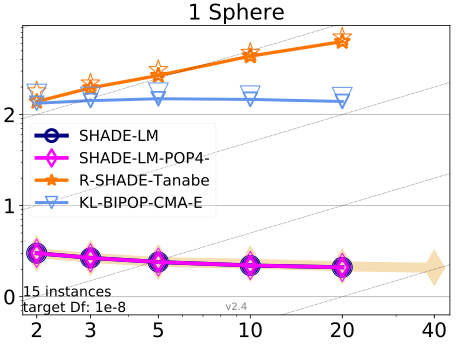
\includegraphics[width=0.238\textwidth]{ppfigs_f001}&
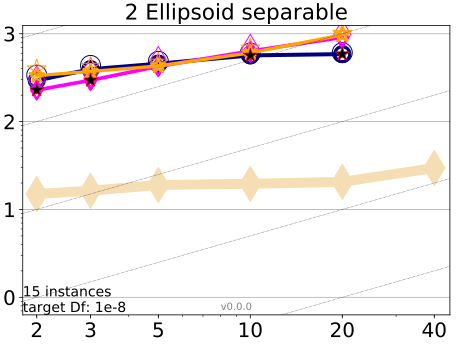
\includegraphics[width=0.238\textwidth]{ppfigs_f002}&
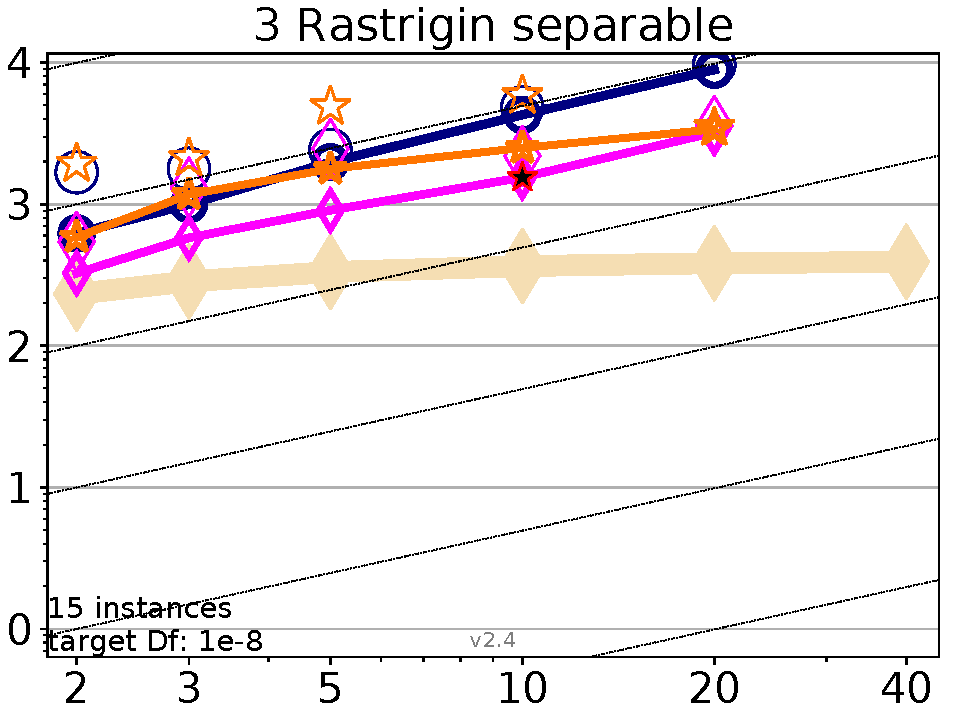
\includegraphics[width=0.238\textwidth]{ppfigs_f003}&
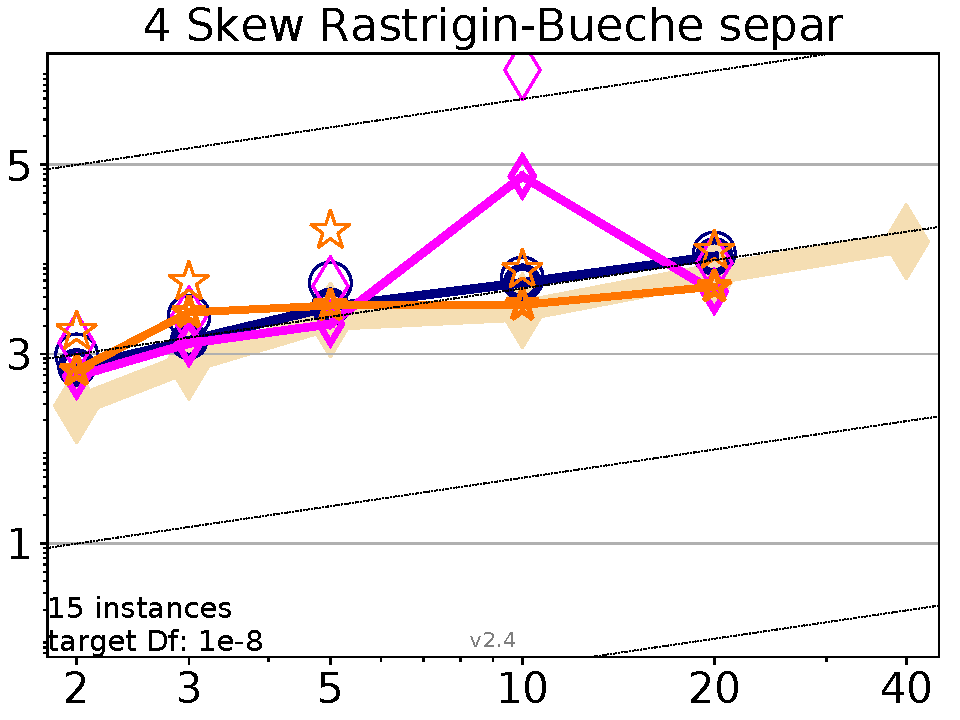
\includegraphics[width=0.238\textwidth]{ppfigs_f004}\\
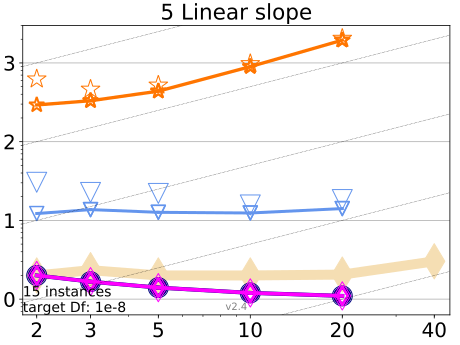
\includegraphics[width=0.238\textwidth]{ppfigs_f005}&
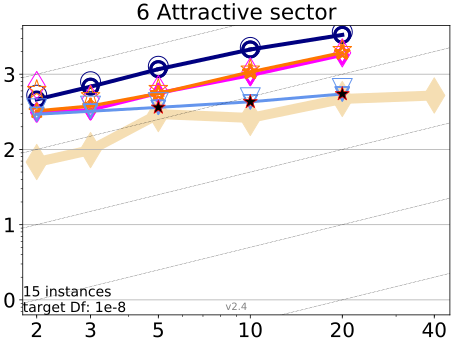
\includegraphics[width=0.238\textwidth]{ppfigs_f006}&
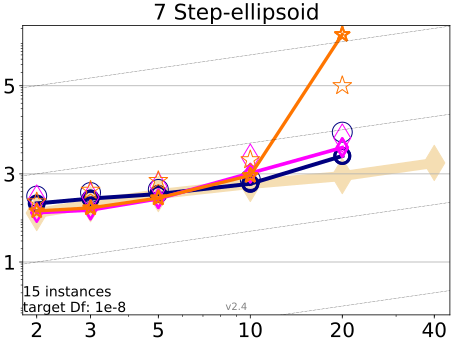
\includegraphics[width=0.238\textwidth]{ppfigs_f007}&
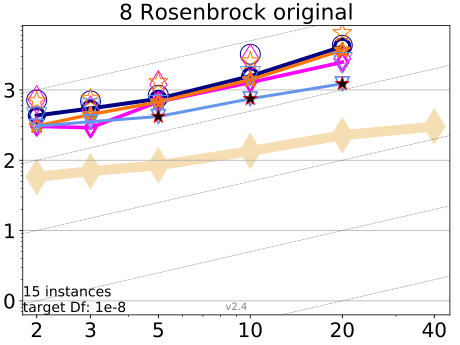
\includegraphics[width=0.238\textwidth]{ppfigs_f008}\\
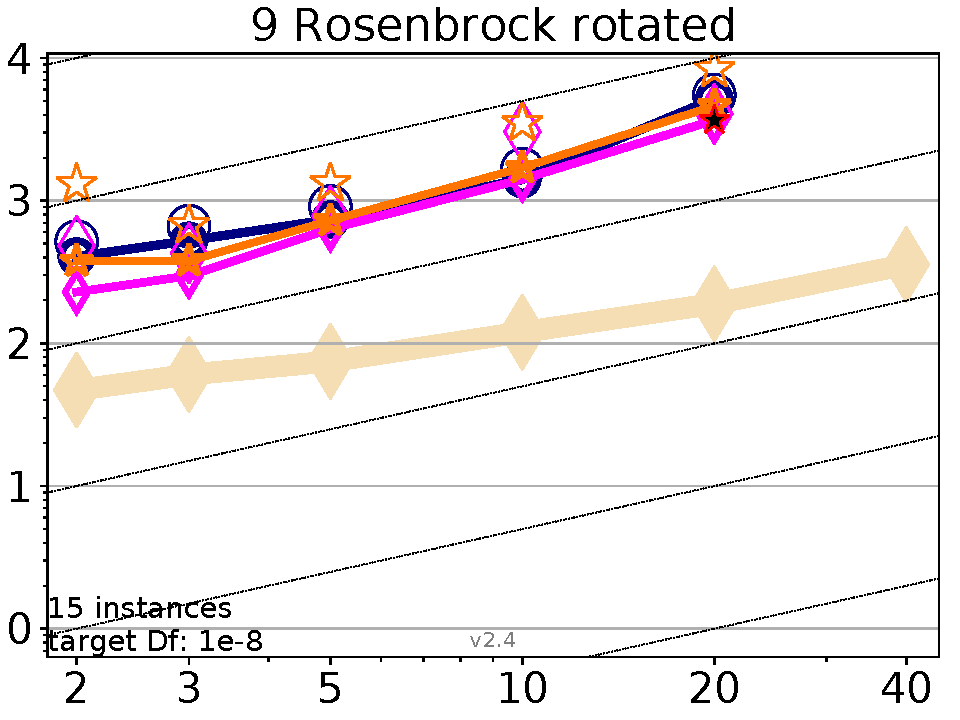
\includegraphics[width=0.238\textwidth]{ppfigs_f009}&
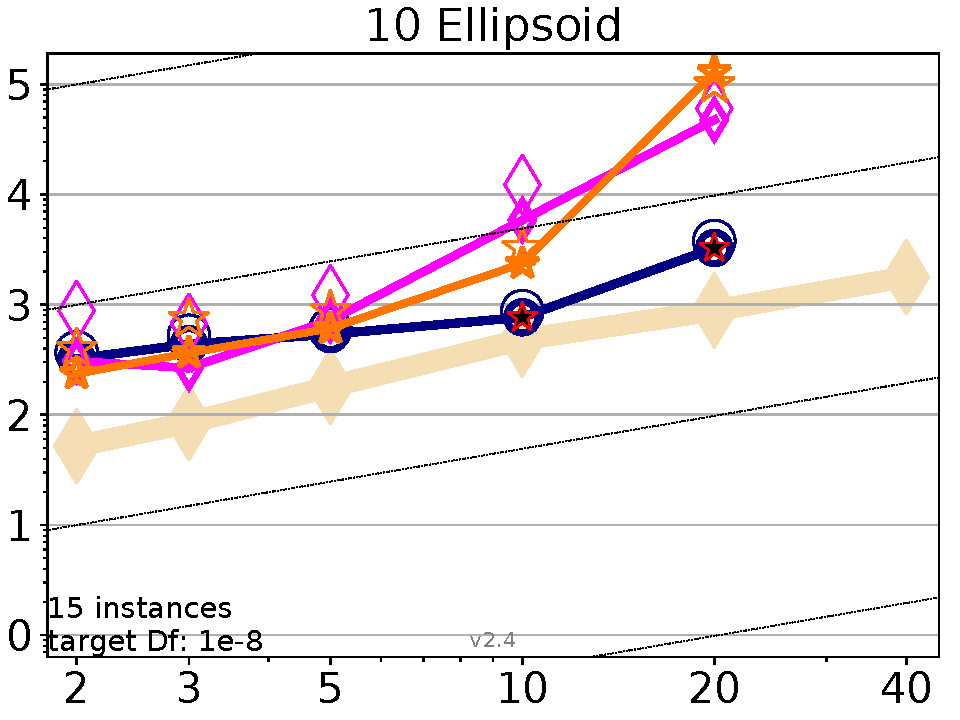
\includegraphics[width=0.238\textwidth]{ppfigs_f010}&
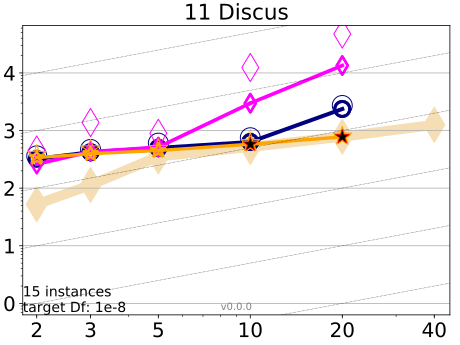
\includegraphics[width=0.238\textwidth]{ppfigs_f011}&
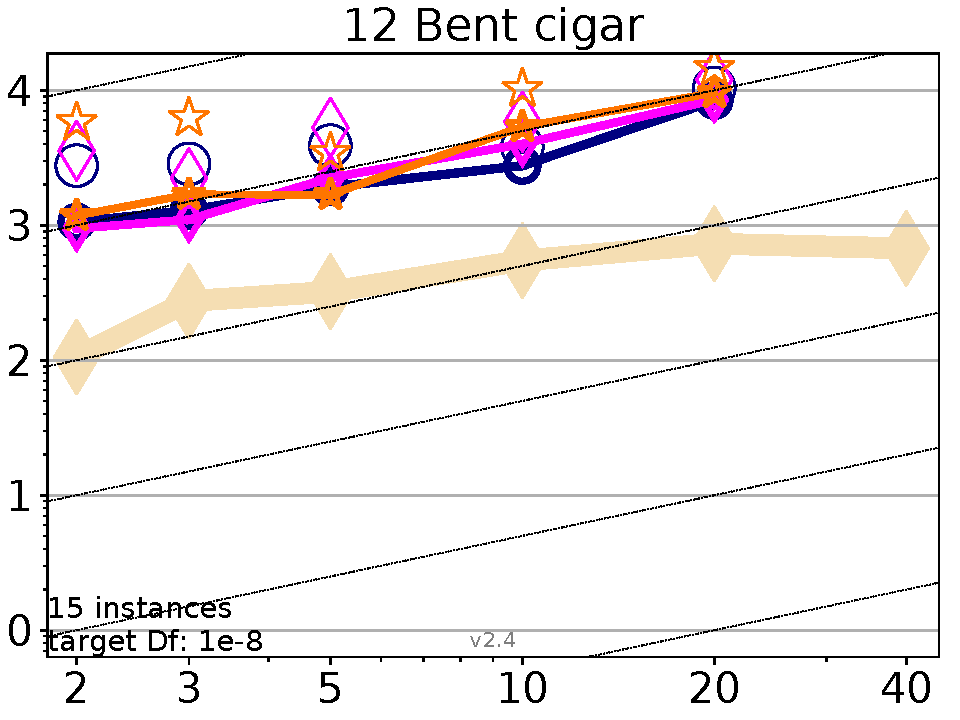
\includegraphics[width=0.238\textwidth]{ppfigs_f012}\\
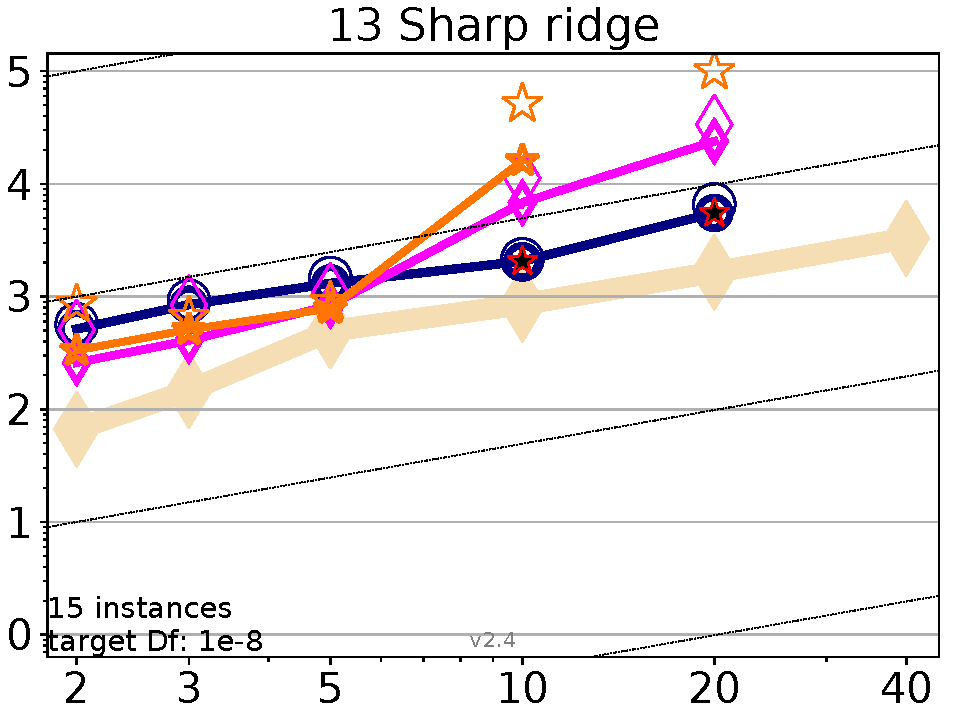
\includegraphics[width=0.238\textwidth]{ppfigs_f013}&
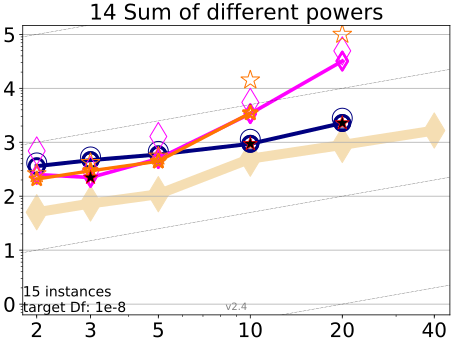
\includegraphics[width=0.238\textwidth]{ppfigs_f014}&
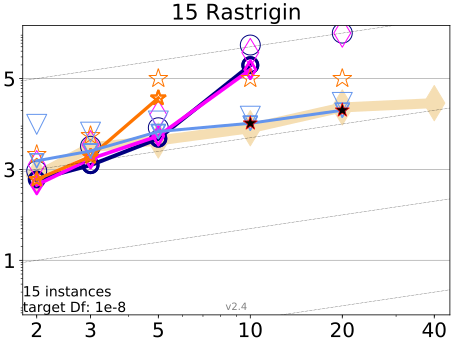
\includegraphics[width=0.238\textwidth]{ppfigs_f015}&
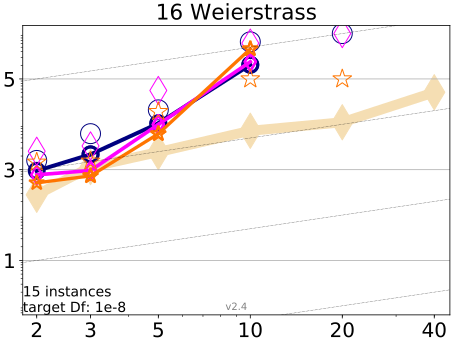
\includegraphics[width=0.238\textwidth]{ppfigs_f016}\\
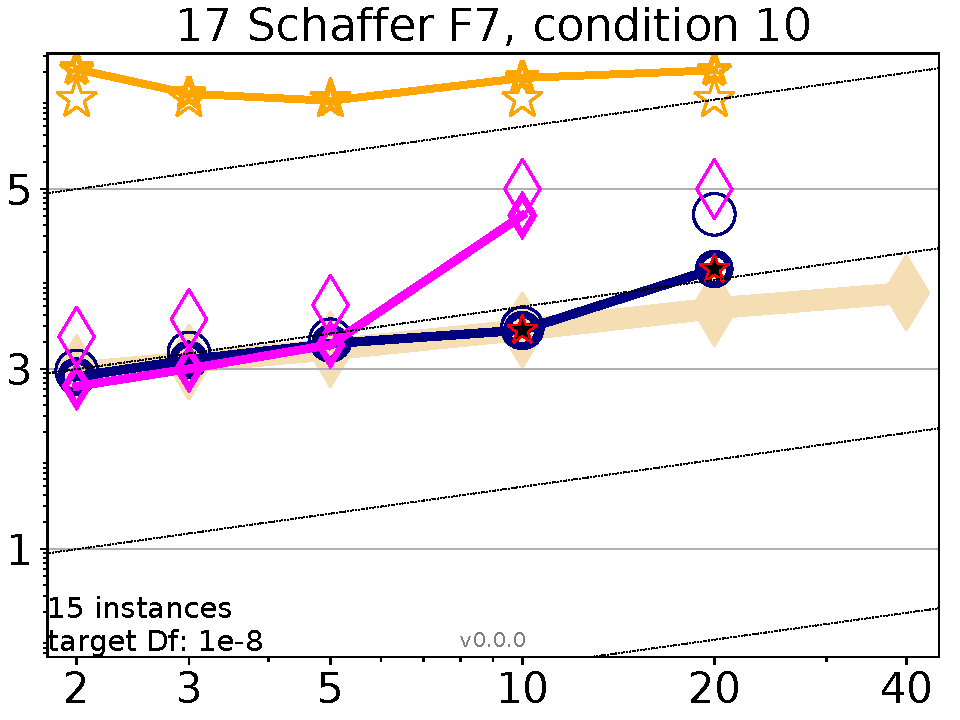
\includegraphics[width=0.238\textwidth]{ppfigs_f017}&
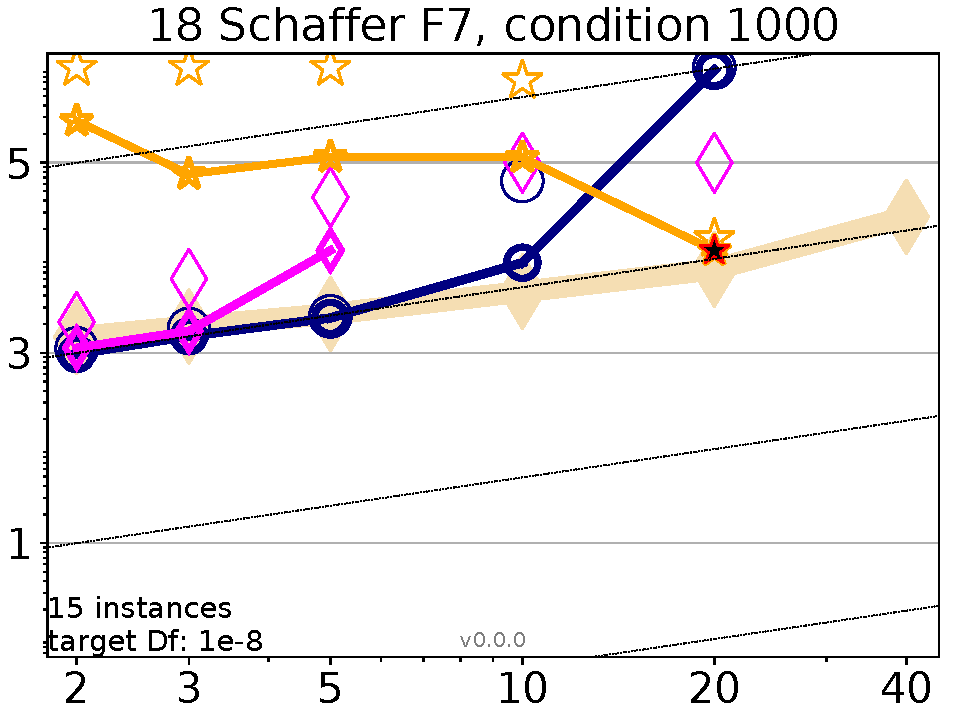
\includegraphics[width=0.238\textwidth]{ppfigs_f018}&
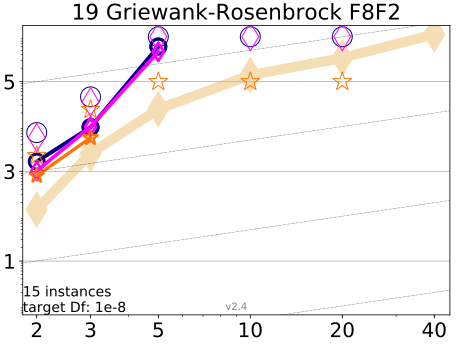
\includegraphics[width=0.238\textwidth]{ppfigs_f019}&
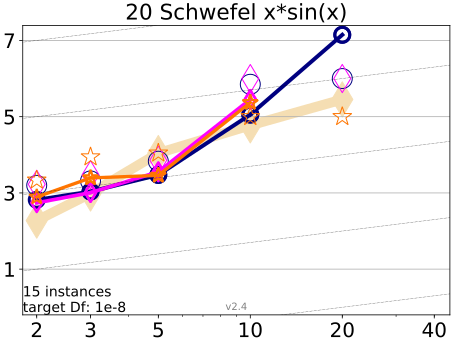
\includegraphics[width=0.238\textwidth]{ppfigs_f020}\\
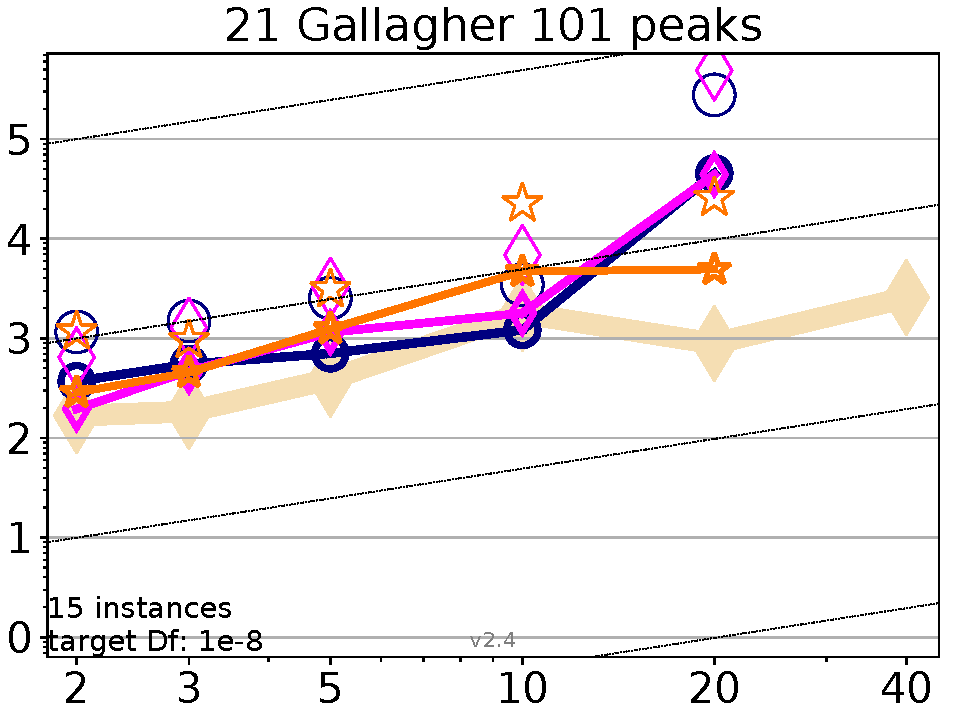
\includegraphics[width=0.238\textwidth]{ppfigs_f021}&
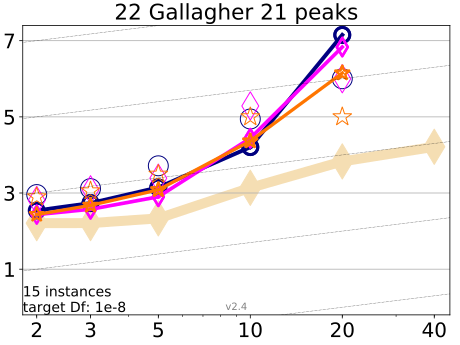
\includegraphics[width=0.238\textwidth]{ppfigs_f022}&
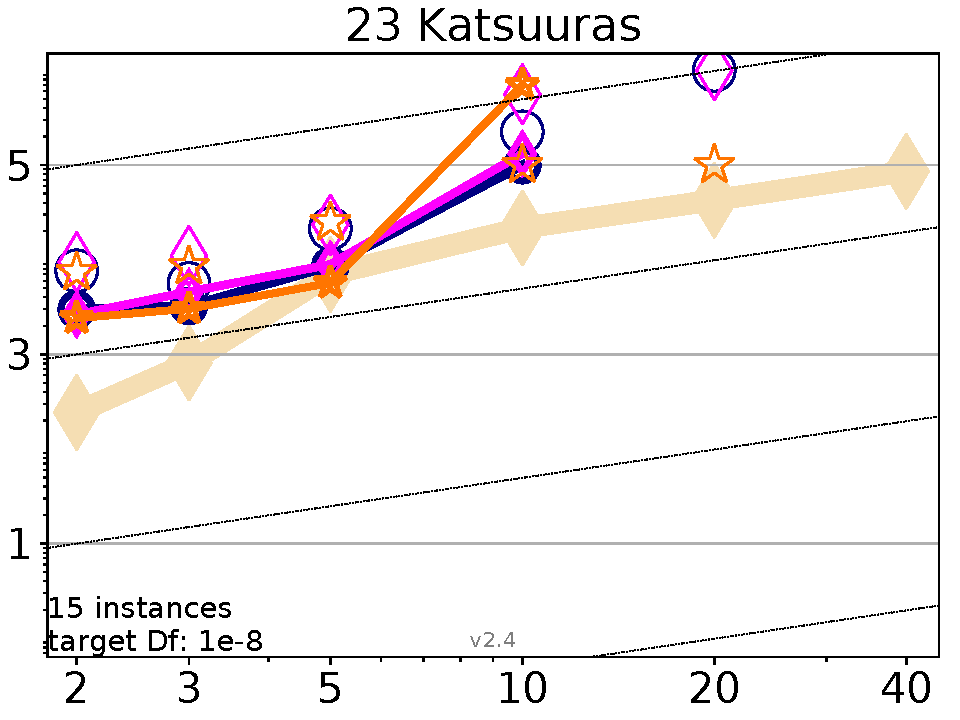
\includegraphics[width=0.238\textwidth]{ppfigs_f023}&
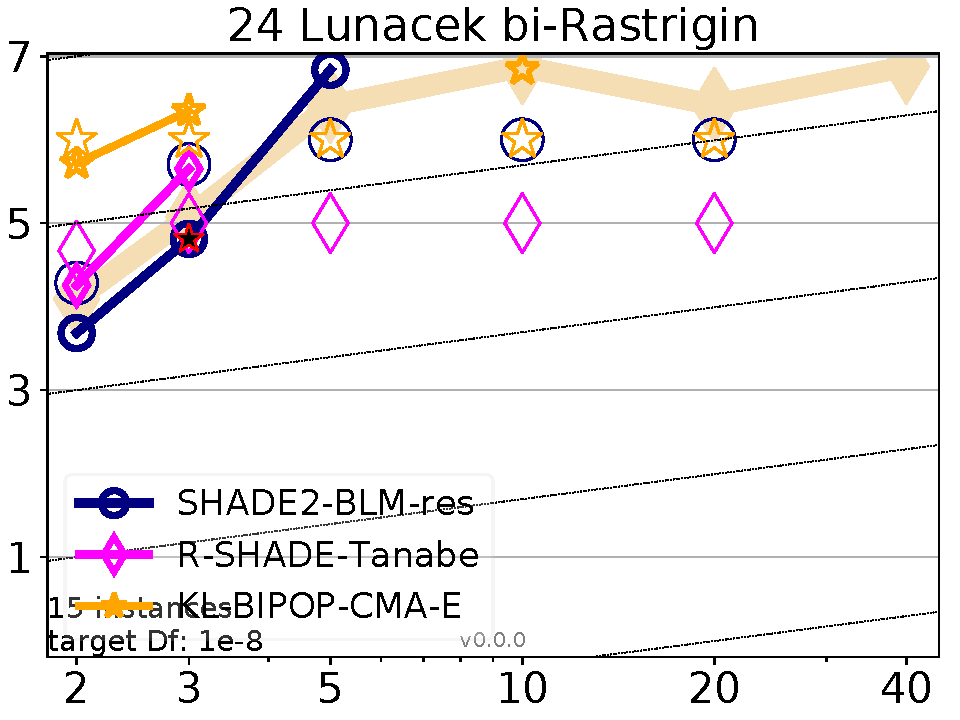
\includegraphics[width=0.238\textwidth]{ppfigs_f024}
\end{tabular}
\vspace*{-0.2cm}
\caption[Expected running time divided by dimension
versus dimension]{
\label{fig:scaling}
% command defined in cocopp_commands.tex:
\bbobppfigslegend{$f_1$ and $f_{24}$}  % \algorithmA can be defined above, see above
}
% 
\end{figure*}



%%%%%%%%%%%%%%%%%%%%%%%%%%%%%%%%%%%%%%%%%%%%%%%%%%%%%%%%%%%%%%%%%%%%%%%%%%%%%%%
%%%%%%%%%%%%%%%%%%%%%%%%%%%%%%%%%%%%%%%%%%%%%%%%%%%%%%%%%%%%%%%%%%%%%%%%%%%%%%%

% Empirical Cumulative Distribution Functions (ECDFs) per function group
% for dimension 5.

%%%%%%%%%%%%%%%%%%%%%%%%%%%%%%%%%%%%%%%%%%%%%%%%%%%%%%%%%%%%%%%%%%%%%%%%%%%%%%%
\newcommand{\rot}[2][2.5]{
  \hspace*{-3.5\baselineskip}%
  \begin{rotate}{90}\hspace{#1em}#2
  \end{rotate}}
\newcommand{\includeperfprof}[1]{% include and annotate at the side
  \input{\bbobdatapath\algsfolder #1}%
  \includegraphics[height=0.24\textheight]{#1}%
  %\raisebox{.12\textheight}{
	%\parbox[b][.24\textheight]{.0868\textwidth}{\begin{scriptsize}
  %  \perfprofsidepanel % this is "\algaperfprof \vfill \algbperfprof \vfill" etc
  %\end{scriptsize}}
	%}
}
%%%%%%%%%%%%%%%%%%%%%%%%%%%%%%%%%%%%%%%%%%%%%%%%%%%%%%%%%%%%%%%%%%%%%%%%%%%%%%%
\begin{figure*}
\begin{tabular}{@{}c@{\hspace*{0.05\textwidth}}c@{}}
 separable fcts & moderate fcts \\
 \includeperfprof{pprldmany_05D_separ} &
 \includeperfprof{pprldmany_05D_lcond} \\ 
ill-conditioned fcts & multi-modal fcts \\
 \includeperfprof{pprldmany_05D_hcond} &
 \includeperfprof{pprldmany_05D_multi} \\ 
 weakly structured multi-modal fcts & all functions\\
 \includeperfprof{pprldmany_05D_mult2} & 
 \includeperfprof{pprldmany_05D_noiselessall} 
 \end{tabular}
\caption{
\label{fig:ECDFs05D}
\bbobECDFslegend{5}
}
\end{figure*}


%%%%%%%%%%%%%%%%%%%%%%%%%%%%%%%%%%%%%%%%%%%%%%%%%%%%%%%%%%%%%%%%%%%%%%%%%%%%%%%
%%%%%%%%%%%%%%%%%%%%%%%%%%%%%%%%%%%%%%%%%%%%%%%%%%%%%%%%%%%%%%%%%%%%%%%%%%%%%%%

% Empirical Cumulative Distribution Functions (ECDFs) per function group
% for dimension 20.

%%%%%%%%%%%%%%%%%%%%%%%%%%%%%%%%%%%%%%%%%%%%%%%%%%%%%%%%%%%%%%%%%%%%%%%%%%%%%%%
\begin{figure*}
 \begin{tabular}{@{}c@{\hspace*{0.05\textwidth}}c@{}}
 separable fcts & moderate fcts \\
 \includeperfprof{pprldmany_20D_separ} &
 \includeperfprof{pprldmany_20D_lcond} \\ 
ill-conditioned fcts & multi-modal fcts \\
 \includeperfprof{pprldmany_20D_hcond} &
 \includeperfprof{pprldmany_20D_multi} \\ 
 weakly structured multi-modal fcts & all functions\\
 \includeperfprof{pprldmany_20D_mult2} & 
 \includeperfprof{pprldmany_20D_noiselessall} 
 \end{tabular}
\caption{
\label{fig:ECDFs20D}
\bbobECDFslegend{20}
}
\end{figure*}


%%%%%%%%%%%%%%%%%%%%%%%%%%%%%%%%%%%%%%%%%%%%%%%%%%%%%%%%%%%%%%%%%%%%%%%%%%%%%%%
%%%%%%%%%%%%%%%%%%%%%%%%%%%%%%%%%%%%%%%%%%%%%%%%%%%%%%%%%%%%%%%%%%%%%%%%%%%%%%%

% Expected runtime (ERT in number of function evaluations)
% divided by the best ERT measured during BBOB-2009 (given in the respective
% first row) for functions $f_1$--$f_{24}$ for dimension 5.

%%%%%%%%%%%%%%%%%%%%%%%%%%%%%%%%%%%%%%%%%%%%%%%%%%%%%%%%%%%%%%%%%%%%%%%%%%%%%%%
\begin{table*}\tiny
%\hfill5-D\hfill~\\[1ex]
{\normalsize \color{red}
\ifthenelse{\isundefined{\algorithmG}}{}{more than 6 algorithms: please split the tables below by hand until it fits to the page limits}
}
\mbox{\begin{minipage}[t]{0.499\textwidth}\tiny
\centering
\pptablesheader
\input{\bbobdatapath\algsfolder pptables_f001_05D} 

\input{\bbobdatapath\algsfolder pptables_f002_05D}

\input{\bbobdatapath\algsfolder pptables_f003_05D}

\input{\bbobdatapath\algsfolder pptables_f004_05D}

\input{\bbobdatapath\algsfolder pptables_f005_05D}

\input{\bbobdatapath\algsfolder pptables_f006_05D}

\input{\bbobdatapath\algsfolder pptables_f007_05D}

\input{\bbobdatapath\algsfolder pptables_f008_05D}

\input{\bbobdatapath\algsfolder pptables_f009_05D}

\input{\bbobdatapath\algsfolder pptables_f010_05D}

\input{\bbobdatapath\algsfolder pptables_f011_05D}

\input{\bbobdatapath\algsfolder pptables_f012_05D}
\end{tabularx}

\end{minipage}
\hspace{0.002\textwidth}
\begin{minipage}[t]{0.499\textwidth}\tiny
\centering
\pptablesheader
\input{\bbobdatapath\algsfolder pptables_f013_05D}

\input{\bbobdatapath\algsfolder pptables_f014_05D}

\input{\bbobdatapath\algsfolder pptables_f015_05D}

\input{\bbobdatapath\algsfolder pptables_f016_05D}

\input{\bbobdatapath\algsfolder pptables_f017_05D}

\input{\bbobdatapath\algsfolder pptables_f018_05D}

\input{\bbobdatapath\algsfolder pptables_f019_05D}

\input{\bbobdatapath\algsfolder pptables_f020_05D}

\input{\bbobdatapath\algsfolder pptables_f021_05D}

\input{\bbobdatapath\algsfolder pptables_f022_05D}

\input{\bbobdatapath\algsfolder pptables_f023_05D}

\input{\bbobdatapath\algsfolder pptables_f024_05D}
\end{tabularx}
\end{minipage}}

 \caption{\label{tab:ERTs5}
 \bbobpptablesmanylegend{dimension $5$}
 }
\end{table*}


%%%%%%%%%%%%%%%%%%%%%%%%%%%%%%%%%%%%%%%%%%%%%%%%%%%%%%%%%%%%%%%%%%%%%%%%%%%%%%%
%%%%%%%%%%%%%%%%%%%%%%%%%%%%%%%%%%%%%%%%%%%%%%%%%%%%%%%%%%%%%%%%%%%%%%%%%%%%%%%

% Expected runtime (ERT in number of function evaluations)
% divided by the best ERT measured during BBOB-2009 (given in the respective
% first row) for functions $f_1$--$f_{24}$ for dimension 20.

%%%%%%%%%%%%%%%%%%%%%%%%%%%%%%%%%%%%%%%%%%%%%%%%%%%%%%%%%%%%%%%%%%%%%%%%%%%%%%%
\begin{table*}\tiny
%\hfill20-D\hfill~\\[1ex]
\mbox{\begin{minipage}[t]{0.499\textwidth}\tiny
\centering
\pptablesheader
\input{\bbobdatapath\algsfolder pptables_f001_20D} 

\input{\bbobdatapath\algsfolder pptables_f002_20D}

\input{\bbobdatapath\algsfolder pptables_f003_20D}

\input{\bbobdatapath\algsfolder pptables_f004_20D}

\input{\bbobdatapath\algsfolder pptables_f005_20D}

\input{\bbobdatapath\algsfolder pptables_f006_20D}

\input{\bbobdatapath\algsfolder pptables_f007_20D}

\input{\bbobdatapath\algsfolder pptables_f008_20D}

\input{\bbobdatapath\algsfolder pptables_f009_20D}

\input{\bbobdatapath\algsfolder pptables_f010_20D}

\input{\bbobdatapath\algsfolder pptables_f011_20D}

\input{\bbobdatapath\algsfolder pptables_f012_20D}
\end{tabularx}
\end{minipage}
\hspace{0.002\textwidth}
\begin{minipage}[t]{0.499\textwidth}\tiny
\centering
\pptablesheader
\input{\bbobdatapath\algsfolder pptables_f013_20D}

\input{\bbobdatapath\algsfolder pptables_f014_20D}

\input{\bbobdatapath\algsfolder pptables_f015_20D}

\input{\bbobdatapath\algsfolder pptables_f016_20D}

\input{\bbobdatapath\algsfolder pptables_f017_20D}

\input{\bbobdatapath\algsfolder pptables_f018_20D}

\input{\bbobdatapath\algsfolder pptables_f019_20D}

\input{\bbobdatapath\algsfolder pptables_f020_20D}

\input{\bbobdatapath\algsfolder pptables_f021_20D}

\input{\bbobdatapath\algsfolder pptables_f022_20D}

\input{\bbobdatapath\algsfolder pptables_f023_20D}

\input{\bbobdatapath\algsfolder pptables_f024_20D}
\end{tabularx}
\end{minipage}}
 \caption{\label{tab:ERTs20}
  \bbobpptablesmanylegend{dimension $20$}
}
\end{table*}


%%%%%%%%%%%%%%%%%%%%%%%%%%%%%%%%%%%%%%%%%%%%%%%%%%%%%%%%%%%%%%%%%%%%%%%%%%%%%%%

\bibliographystyle{ACM-Reference-Format}
\bibliography{./bbob}  % bbob.bib is the name of the Bibliography in this case

\clearpage % otherwise the last figure might be missing


\end{document}
